\documentclass[a4paper]{article}

\usepackage[english]{babel}
\usepackage[utf8]{inputenc}
\usepackage{amsmath}
\usepackage{graphicx}
\usepackage{grffile}

\title{Distributed Control of Wide Area Power System}

\author{}

\date{\today}

\begin{document}
\maketitle


\section{Introduction}
In this experiment, security attacks are simulated on the communication links of a wide- area power system, disrupting the flow of measurement data from the machines and control input to the machines. This temporary disconnect in the network may cause the dynamic system performance to deteriorate or even cause instability.The aim of the study is to find a sensitivity plot which identifies the scenarios which would result in instability of the system or deterioration in the system performance and to determine the regions of safe operation.
\section{Test Bed Architecture}
\subsection{Power System Simulation}

\subsubsection{ RTDS HIL Model}
 
A multi machine wide area power system model is designed in RSCAD. The model is loaded on to the RTDS (Real Time Digital Simulator), an Hardware in loop simulator, to run real time simulations. The generator states are measured from the internal bus with a PMU (Phasor Measurement Unit) during the simulations. The PMUs are connected to the ports in GTAO(Giga-Transceiver Analogue Output) Card of the RTDS.

The PMU measures the bus voltage, phase angle and frequency. These measurement data from all the PMUs are then forwarded to the PDC(Phasor Data Concentrator). The PDC combines the data from all the PMUs based on their synchronized timestamp. PDC communicates the measurement signal as an IEEE C37.118 message to the base station (computer) over the ethernet as UDP datagrams. In order to implement the control the PDC measurement data is forwarded to the controllers present at the DETER nodes through the Internet using UDP communication.

\subsubsection{MATLAB Model}

For testing purposes a six machine wide area power system model was designed in MATLAB.The states of the machine are directly measured and communicated to the network controller. In order to make the software simulation closer to the real time simulation a first order hold is implemented in the closed loop control signal (i.e. the value of the control input from the previous time sample is used until a new sample arrives).

\subsection{Network Structure}
 
 The PDC measurement data is received at the base station (GILIA machine) using the PDC Assistant software. The measurement data is transmitted at a 60Hz data frequency in the Local Area Network. This data message is forwarded to the FEDD virtual machine in GILIA through NAT(Network Address Translator). The FEDD VM acts as gateway node to  communicate with the DETER Network. A federated experiment is created with the FEDD VM as an external desktop node and all the other nodes are present within the DETER network. Each deter node represents a individual machine.
 
 The FEDD node routes the received data messages to the deter node where the IEEE C37.118 message is decoded based on the initial configuration message. The standard IEEE message is decoded to obtain the phase angle and frequency data from each machine. The states of each machine is forwarded to individual nodes which resembles the machines. All machine nodes are interconnected with each other, in order to share/communicate the states with all the machines, in a full graph network structure. A LQR controller is designed considering the linearized model of the power system and accommodating the delays induced by the data transfer in the network. The feedback gains of each machine calculated from the LQR design are fed into the the nodes and each node individually generates the control signal with the measurement data of states of all the machines.

 The calculated control inputs are then routed back to the FEDD VM. The FEDD VM transmits the control inputs back to the RTDS Model by sending them as UDP packets to the GTNET card using socket protocol. In case of the MATLAB simulations the control inputs are forwarded directly to the matlab program. 
 


\begin{figure}
\centering
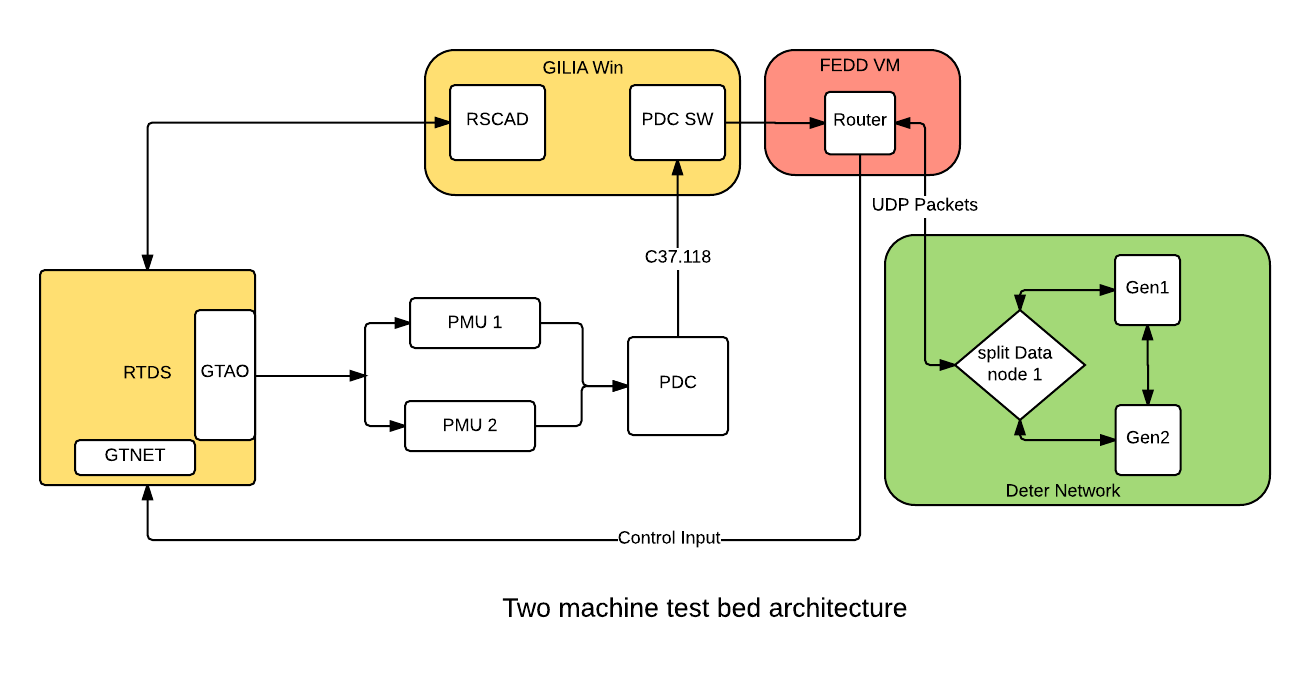
\includegraphics[width=1\textwidth]{Test_bed_Architecture.png}
\caption{\label{fig:testbed}The Test bed architecture}
\end{figure}

\section{Mathematical Model and Control Design}
\subsection{Power System Model}
Let us consider a power system network with n generators distributed into multiple areas. The Internal voltage of any $i$th generator is given by $\hat{E_{i}} =E_{i}\angle\delta_{i}, i = 1:n$. Each synchronous generator may be modelled by a set a third order algebraic differential equations,
\begin{equation}
\label{eq1}
\begin{split}
\dot{\delta_{i}}&={\omega_{s}}\\
2H_{i}\dot{{\omega_{i}}} &= {P}_{mi}-D_{i}({\omega_{i}-\omega_{s}})-P_{i}^{G} \\
\tau_{i}\dot{E_{i}} &= -\frac{x_{di}}{x'_{di}}+ \frac{x_{di}-x^{'}_{di}}{x^{'}_{di}}V_{i}cos(\delta_{i}-theta_{i}) +\hat{E_{Fi}}\\
P_{i}^{G} &=\frac{{E}_{i}{V}_{i}}{{x}_{di}^{'}}{\sin}({\delta}_{i} -{\theta}_{i})\\
\end{split}
\end{equation}

where, the states $\delta_{i},\omega_{i}$ and $E_{i}$ are respectively, the generator phase angle(radians), angular velocity of the rotor(rad/sec) and quadrature-axis internal emf; $\omega_{s}$ is the synchronous frequency of 120$\pi$ radians/sec; $P_{i}^{G}$ is the active power produced by the $i$th generator; $2H_{i}$ is the inertia constant(seconds), $D_{i}$ is the generator damping, ${x}_{di}^{'}$ is the direct axis transient reactance; $P_{mi}$ is the mechanical power input to the $i$th turbine(MW). $\tau_{i}$ is the excitation time constant(seconds);$x_{di}$, $x'_{di}$ and $x_{qi}$ are the direct-axis salient reactance, direct axis transient reactance and quadrature axis salient reactance (all in ohms), respectively. The control variable is the field voltage $E_{Fi}$, which is the variation of $\hat{E_{Fi}}$ from the equilibrium point.\\
Firstly to linearize the non-linear swing equations,consider a small perturbation over an existing equilibrium $(\delta_{i0},\omega_{i0}),i = 1:n$. The overall linearized small signal model of the power system can be expressed as

\begin{equation}
\label{eq2}
\begin{bmatrix}
{\Delta}\dot{{\delta}}(t)\\
2H{\Delta}\dot{{\omega}}(t)\\
T{\Delta}\dot{E(t)}\\
\end{bmatrix} =
\begin{bmatrix}
0 &I &0\\
-L &-D &-P\\
K &0 &J\\
\end{bmatrix}
\begin{bmatrix}
{\Delta}{\delta}(t)\\
{\Delta}{\omega}(t)\\
{\Delta}E(t)\\
\end{bmatrix} +
\begin{bmatrix}
0 0\\
I 0\\
0 I\\
\end{bmatrix}
\begin{bmatrix}
\Delta P_{m}\\
\Delta E	_{F}\\
\end{bmatrix}
\end{equation}
where, $\Delta{\delta} = col(\Delta{\delta}_{1},\ldots,\Delta{\delta}_{n})$, $\Delta{\omega} = col(\Delta{\omega}_{1},\ldots,\Delta{\omega}_{n})$, $H = diag(H_{1},\ldots,H_{2})$, $\Delta P_{m} = col(\Delta P_{m1},\ldots,\Delta P_{mn})$, $\Delta E_{F} = col(\Delta E_{F1},\ldots,\Delta E_{Fn})$ and $T = diag(\tau_{1},\ldots,\tau_{n})$ .The turbine mechanical power $\Delta P_{m}$ typically has a much lower bandwidth than needed for oscillation damping. Therefore for wide area control designs, $\Delta P_{m}$ is treated as zero, and   The continuous time state space model of the linearized small signal system can be represented by \eqref{eq3}. The control input $\Delta E_{F}$ is designed using PMU data feedback.
\begin{equation}\label{eq3} \dot{X}(t) = A_{c}X(t) +B_{c}U(t) \end{equation}
where $A_{c}$ - Continuous time state Matrix $B_{c}$ - Continuous time Input matrix and $X$ is the state vector.
The practical implementation of a power system controller in a distributed network would be in the discrete-time.The states from the power system are measured using the PMUs at a sampling rate of one sample per $\tau$ seconds. The sampling interval of the states is $\tau$ seconds. The discrete time model of the system is given by \eqref{eq4}

\begin{equation}
\label{eq4}
\begin{split}
X[k+1] &= A_{d}X[k] + B_{d}U[k]\\ 
A_{d} &= e^{A_{c}\tau}\\
B_{d} &= \int_{0}^{t = \tau}{e^{A_{c}t} dt} B_{c}\\
\end{split}
\end{equation}

where, $A_{d}$ is the discrete-time state matrix and $B_{d}$ is the discrete-time input matrix. The discrete time state space model is given by \eqref{eq4}.\\
 Since the controller is being implemented on a distributed network, the states of all the machines at time instant $k$ are not readily available at time $t= k$. The states of $i$th machine arrives to every other controller node after a random communication delay. The maximum delay threshold of a network is a characteristic of the communication network. Let us assume $h$ to be the maximum delay threshold of our network. This implies that in ideal conditions when all links are operational the states of the machines reach every other controller node within $h$ seconds. The control input cannot be evaluated until all the states are available, hence the control input for time instant $k$ will be available only at $t = k+h$. The control input for the period $t = [k,k+h)$ will be the control input calculated at the previous time instant, $U[k-1]$. The effective control input $u_{i}(t)$  for a single sampling time duration $ k<t<k+1$ is represented by

\begin{equation}
\label{eq5}
u_{i}[t]  = \begin{cases} u_{i}[k-1] & \quad \text{, } k<t<k+h\\ u_{i}[k] & \quad \text{, } k+h<t<k+1\\ \end{cases}
\end{equation}
The effective discrete time state space model can be written as,
\begin{equation}
\label{eq6}
\begin{split}
X[k+1] &= AX[k] + B_{1}U[k-1] +B_{2}U[k]\\
B_{1}  &= \int_{0}^{t = h}e^{At}B_{c}dt \hspace{3pt} 
B_{2}  = \int_{h}^{t = \tau}e^{At}B_{c}dt\\
\end{split}
\end{equation}
By defining an augmented state $Z[k] = [X[k] $ $U[k-1]]^{T}$, \eqref{eq6} can be written as:
\begin{equation}
\begin{split}
\label{eq7}
Z[k+1] &= 
\begin{bmatrix}
A & B_{1}\\
0 & 0\\
\end{bmatrix} 
\begin{bmatrix}
X[k]\\
U[k-1]
\end{bmatrix}+
\begin{bmatrix}
B_{2}\\
I
\end{bmatrix}\\&=
\hat{A}Z[k] + \hat{B}U[k]
\end{split}
\end{equation}
A Linear Quadratic Regulator(LQR) controller is designed to control the discrete time system. The LQR optimizes the quadratic cost function $J$,
\begin{equation}
\label{eq8}
J = \sum_{k = 0}^{\infty}Z_{k}^{T}QZ_{k} +U_{k}^{T}RU_{k}
\end{equation}
where $Q$ and $R$ are the design parameters. The control input $U[k]$ from the control law can be written as,
\begin{equation}
\label{eq9}
U[k] = KZ[k] = K_{0}X[k] +L_{0}U[k-1]
\end{equation}
where K is the feedback gain resulting from the LQR control design.

\subsection{Network Implementation}
\begin{figure}
\centering
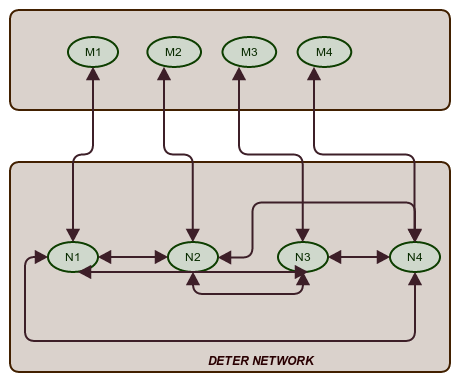
\includegraphics[width=0.7\textwidth]{Network_Setup.png}
\caption{\label{fig:table} Network Topology}
\end{figure}
This LQR controller is implemented in a distributed network system. The states from the machines are transmitted to the deter nodes and each node evaluates the control input for the respective machine and transmits back to the machine. In order to evaluate the control input all the nodes require the states from all the other machines at every sampling instant.Hence the network will be a full graph structure where all nodes are connected with each other, the graph for a $n$ machine model can be denoted by G. A full graph will have all the elements in the matrix to be 1.when there is a link between nodes $i$ and $j$ down/broken the $G[i,j] = G[j,i] = 0$
\begin{equation}
G = 
\begin{pmatrix}
1 &1 &\cdots &1\\
1 &1 &\cdots &1\\
\vdots &\vdots &\ddots &\vdots\\
1 &1 &\cdots &1\\
\end{pmatrix}_{nxn}
\end{equation}
The control input of the $i$th machine at any time instant $l$ , $u_{i}(l)$ given by , is evaluated by using the measured states of all the machines.
\begin{equation}
\label{eq12}
u_{i}[k] = (K_{0i}\circ G_{i}) X[k] + L_{0i}U[k-1]
\end{equation}
where, $K_{0i}$,$L_{0i}$ and $G_{i}$ are the $i$th row of the state feedback matrix $K_{0}$, the gain matrix $L_{0}$ corresponding to the previous input and Graph matrix $G$ respectively.\\


\section{Simulation and Testing}

A number of simulations can be run in the test bed to study the stability and dynamics of the multi machine wide area power system when there is a security attack (denial of service) on the links connecting the generator nodes.The variables considered in the test scenarios are 
\begin{enumerate}
\item duration of attack
\item Location of attack ( link)
\item time identity (i.e. the time of attack after the start of simulation).
\end{enumerate}

A denial of service attack is simulated by using the capabilities of deter network, by flooding the link with enormous amount of data. A typical attack  lasts for a specific number of time samples either on one or multiple links. During an attack the graph of the network is not a full graph and can be represented by $G_{A}$, if the links between nodes m and n are attacked the elements $G_{A}(m,n) = G_{A}(n,m) = 0$. For example if link between node 2 and node 3 is attacked the network graph of a 4 machine system will be,
\begin{equation}
G_{A} = 
\begin{pmatrix}
1 &1 &1 &1\\
1 &1 &0 &1\\
1 &0 &1 &1\\
1 &1 &1 &1\\
\end{pmatrix}_{4x4}
\end{equation}

We have 3 different mitigation strategies to reduce the effects of the loss of data due to attacks on the links.The strategies are
\begin{enumerate}
\item Strategy 1: Skip strategy
\item Strategy 2: Zero Order Hold
\item Strategy 3: State Estimation
\end{enumerate}
below is a list of scenarios, 
\subsection{Test Scenarios} 
\subsection{Scenario-1: Ideal Case (No Attack)}
Under ideal conditions, all the communication links between the deter nodes are functional and the states of all the machines reach every other machine within the maximum delay threshold $h$. The deter nodes then evaluate the control input based on states of the machines and the control input at previous time instant as shown in \eqref{eq12}. 
\subsubsection{Scenario-2 : Attack on single link}
In this case a denial of service attack is simulated on each link individually. The network graph will now have two zero elements. The attack is simulated for a specific number of time samples, $n$, where $n=1,2,3,4,5$. The control input $u_{i}[k]$ of $i$th machine can be written as,

where,$K_{0i}$ and $L_{0i}$ are the $i$th rows of the feedback gain matrices corresponding to the states of the machines and the previous control inputs,$G_{Ai}$ is the graph of the network during attack.
\subsubsection{ Scenario-2 : Attack on multiple links}
The Denial of service attack is simulated on multiple links simultaneously. The network graph will have multiple zero elements. The attack is simulated for $n$ time samples where $n = 1,2,3,4,5$.

\subsubsection{ Scenario-3 : Attack on links at different time identities}
Performing both the Scenario 1 and Scenario 2 at different time instants of the simulation.(e.g. at the start of the simulation, towards the end of the simulation where the system  reaches steady state, at half the settling time).
\subsection{ Mitigation Strategies}
\subsubsection{Strategy 1: Skip Strategy}
According to skip strategy the states of the machines  are assumed to be zero if they are not available to the node before the threshold delay time, $h$. The control input is calculated with zero value for the missing states and can be written as,
\begin{equation}
u_{i}[k] = (K_{0i}\circ G_{Ai}) X[k] + L_{0i}u_{i}[k-1] 
\end{equation}
\subsubsection{Strategy 2: Zero Order Hold}
In case of strategy 2 the states of the machines at previous instant of time are stored at each node. If state $x_{i}[k]$, the state of $i$th machine at time instant k, does not arrive within the threshold $h$, then $x_{i}[k-1]$ is used to evaluate the control input.(i.e.) $x_{i}[k] = x_{i}[k-1]$. If the state of $i$th machine is not available for $n$ consecutive time samples then $x_{i}[k] = x_{i}[k-n]$, where $n = 1,2,3,4,5$. The control input evaluated at the node can be represented as,
\begin{equation}
u_{i}[k+n] = (K_{0i}\circ G_{Ai}) X[k+n] + L_{0i}u_{i}[k-1+n] + K_{0mi}x_{m}[k-n]
\end{equation}

\subsubsection{Strategy 3: State Estimation}
In case of strategy 3 the states of the machines and previous control input values are stored at each node. If state $x_{m}[k]$, the state of $m$th machine at time instant $k$, does not arrive within the threshold $h$, then $x_{m}[k]$ is estimated by solving the discrete time state space of the dynamic system in \eqref{eq7}. The control input is then evaluated by using this estimated state value for the missing state. The control input can be written as,
\begin{equation}
u_{i}[k] = (K_{0i}\circ G_{Ai}) X[k] + L_{0i}u_{i}[k-1] + K_{0mi}\hat{x_{m}}[k]
\end{equation}
where $K_{0mi}$ is the $(i,m)$th element of the feedback gain matrix $K_{0}$ and $\hat{x_{m}}[k]$ is the estimated value of the state of $m$th machine. This strategy would reduce the difference between the ideal case control input and estimated control input during a security attack.
\subsection{Senstivity Plot}
With the results from running the simulations for all the above test cases we will be able to identify the cases/scenarios when the system is stable, unstable and the performance is degraded. With this information a sensitivity plot as shown in fig(3) for different time identities can be plotted. These plots can be used to identify the stability regions.

\begin{figure}
\centering
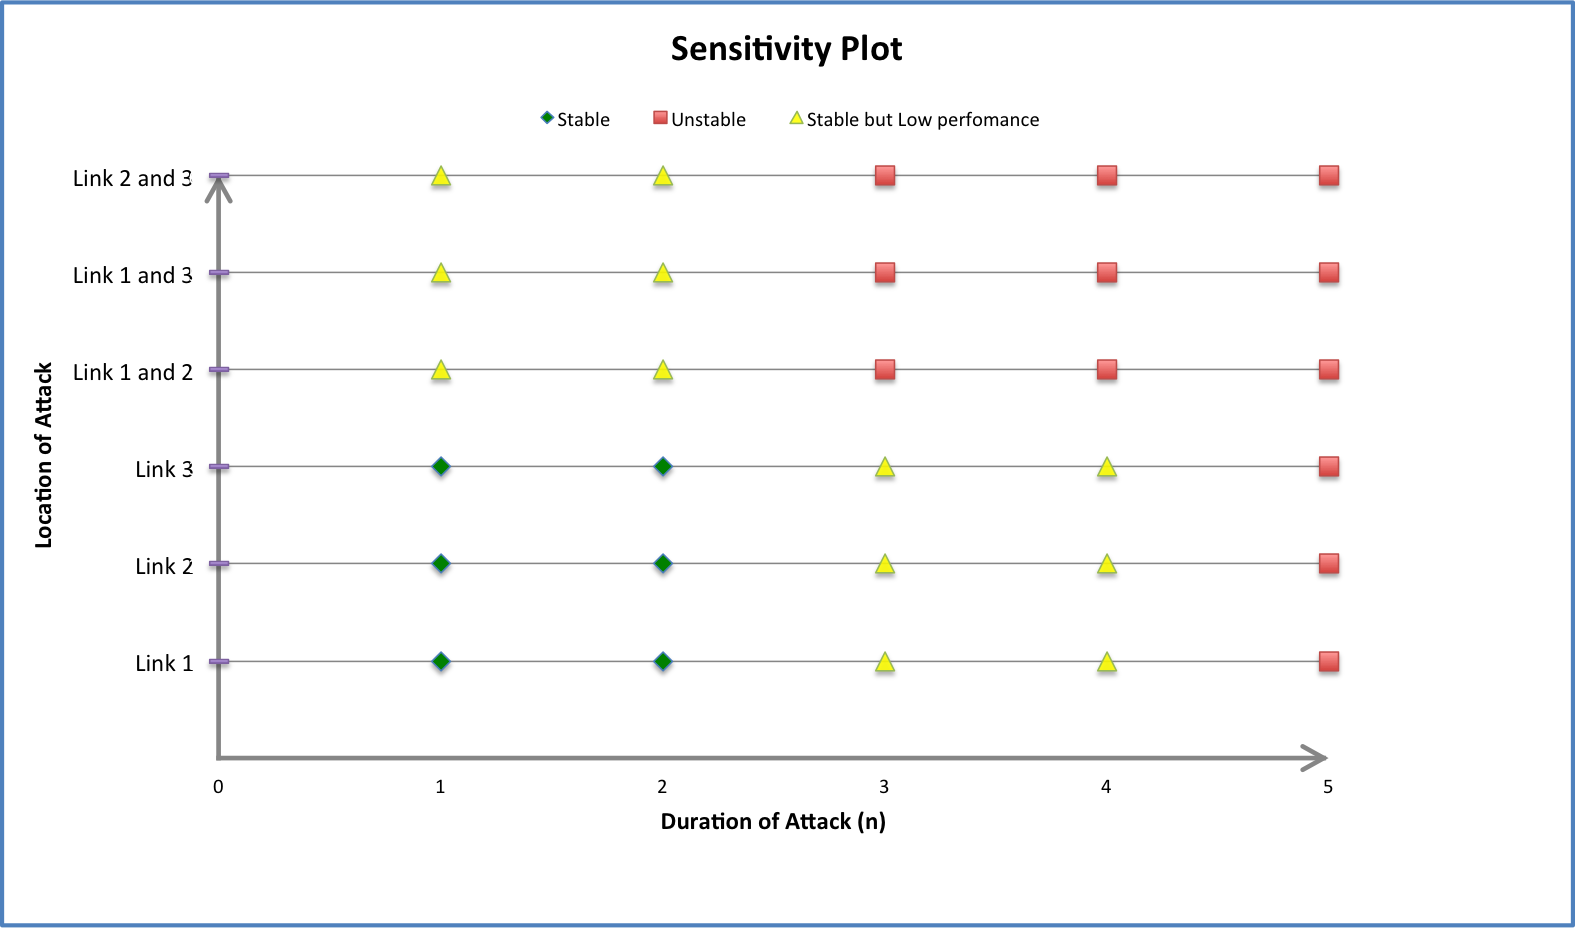
\includegraphics[width=0.9\textwidth]{sensitivity_plot2.png}
\caption{\label{fig:plot} Plot illustrating the stability region}
\end{figure}

\end{document}
